
\lecture{Confidence Intervals Part II}{confidence-interval-II}
\section{Review of Confidence Intervals}

\title{Confidence Intervals}
\subtitle{Review of What We Have Done}

%\author{Kelly Black}
%\institute{Clarkson University}
\date{12 March 2013}

\begin{frame}
  \titlepage
\end{frame}

\begin{frame}
  \frametitle{Outline}
  \tableofcontents[pausesection,hideothersubsections,sectionstyle=show/hide]
\end{frame}


\subsection{Clicker Quiz}


\iftoggle{clicker}{%
  \begin{frame}
    \frametitle{Clicker Quiz}

    Thirty-one medium sized companies are sampled from a given sector. For
    each company the amount of money spent for research per year is
    sampled. The sample mean for expenditures is 1.3 million dollars
    with a sample standard deviation of 0.18 million dollars. What is
    the 90\% confidence interval for the mean?

    \vfill


    \begin{tabular}{l@{\hspace{3em}}l@{\hspace{3em}}l@{\hspace{3em}}l}
      A: 1.221 to 1.379 million  & B: 1.234 to 1.366 million  & C: 1.245 to 1.355 million
    \end{tabular}

    \vfill
    \vfill
    \vfill

  \end{frame}
}

\subsection{Confidence Intervals}


\begin{frame}

  \centerline{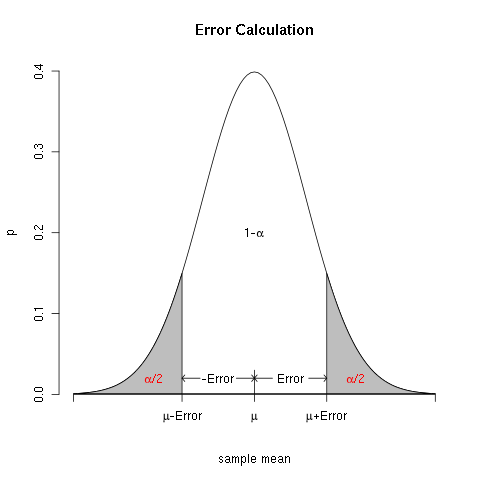
\includegraphics[width=6cm]{img/confidenceInterval}}

  \begin{columns}[T]

    \begin{column}[T]{0.5\textwidth}
      The R.V. $X$ has mean $\mu$ and standard deviation $\sigma$.

      The sample mean, $\bar{x}$ has mean $\mu$ and standard deviation
      $\frac{\sigma}{\sqrt{n}}$.

    \end{column}

    \begin{column}[T]{0.5\textwidth}
      The sample proportion has mean $p$ and standard deviation
      $\sqrt{\frac{p(1-p)}{n}}$.

      %\vfill
    \end{column}

  \end{columns}


\end{frame}



\begin{frame}
  \frametitle{The Confidence Interval}

  \begin{columns}
    \column{0.25\textwidth}
    \begin{definition}
      The \textit{confidence interval} is an interval that likely
      includes the true mean.
    \end{definition}

    \column{0.75\textwidth}

    % Graphic for TeX using PGF
% Title: /home/black/write/class/stat/stat282-12/class/img/confidenceIntervalDist.dia
% Creator: Dia v0.97.2
% CreationDate: Mon Mar  4 12:17:58 2013
% For: black
% \usepackage{tikz}
% The following commands are not supported in PSTricks at present
% We define them conditionally, so when they are implemented,
% this pgf file will use them.
\ifx\du\undefined
  \newlength{\du}
\fi
\setlength{\du}{15\unitlength}
\begin{tikzpicture}[thick,scale=0.6, every node/.style={scale=0.6}]
\pgftransformxscale{1.000000}
\pgftransformyscale{-1.000000}
\definecolor{dialinecolor}{rgb}{0.000000, 0.000000, 0.000000}
\pgfsetstrokecolor{dialinecolor}
\definecolor{dialinecolor}{rgb}{1.000000, 1.000000, 1.000000}
\pgfsetfillcolor{dialinecolor}
\definecolor{dialinecolor}{rgb}{1.000000, 1.000000, 1.000000}
\pgfsetfillcolor{dialinecolor}
\fill (9.875000\du,2.350000\du)--(9.875000\du,5.050000\du)--(16.525000\du,5.050000\du)--(16.525000\du,2.350000\du)--cycle;
\pgfsetlinewidth{0.100000\du}
\pgfsetdash{}{0pt}
\pgfsetdash{}{0pt}
\pgfsetmiterjoin
\definecolor{dialinecolor}{rgb}{0.000000, 0.000000, 0.000000}
\pgfsetstrokecolor{dialinecolor}
\draw (9.875000\du,2.350000\du)--(9.875000\du,5.050000\du)--(16.525000\du,5.050000\du)--(16.525000\du,2.350000\du)--cycle;
% setfont left to latex
\definecolor{dialinecolor}{rgb}{0.000000, 0.000000, 0.000000}
\pgfsetstrokecolor{dialinecolor}
\node at (13.200000\du,3.495000\du){Read the };
% setfont left to latex
\definecolor{dialinecolor}{rgb}{0.000000, 0.000000, 0.000000}
\pgfsetstrokecolor{dialinecolor}
\node at (13.200000\du,4.295000\du){Problem};
\pgfsetlinewidth{0.100000\du}
\pgfsetdash{}{0pt}
\pgfsetdash{}{0pt}
\pgfsetbuttcap
{
\definecolor{dialinecolor}{rgb}{0.000000, 0.000000, 0.000000}
\pgfsetfillcolor{dialinecolor}
% was here!!!
\pgfsetarrowsend{stealth}
\definecolor{dialinecolor}{rgb}{0.000000, 0.000000, 0.000000}
\pgfsetstrokecolor{dialinecolor}
\draw (13.257154\du,5.099002\du)--(13.327646\du,6.824488\du);
}
\pgfsetlinewidth{0.100000\du}
\pgfsetdash{}{0pt}
\pgfsetdash{}{0pt}
\pgfsetmiterjoin
\pgfsetbuttcap
{
\definecolor{dialinecolor}{rgb}{0.000000, 0.000000, 0.000000}
\pgfsetfillcolor{dialinecolor}
% was here!!!
\pgfsetarrowsend{stealth}
{\pgfsetcornersarced{\pgfpoint{0.000000\du}{0.000000\du}}\definecolor{dialinecolor}{rgb}{0.000000, 0.000000, 0.000000}
\pgfsetstrokecolor{dialinecolor}
\draw (8.390350\du,9.409510\du)--(8.390350\du,9.400000\du)--(6.958340\du,9.400000\du)--(6.958340\du,11.745900\du);
}}
\definecolor{dialinecolor}{rgb}{1.000000, 1.000000, 1.000000}
\pgfsetfillcolor{dialinecolor}
\fill (6.958337\du,11.745900\du)--(10.124835\du,14.536969\du)--(6.958337\du,17.328039\du)--(3.791840\du,14.536969\du)--cycle;
\pgfsetlinewidth{0.100000\du}
\pgfsetdash{}{0pt}
\pgfsetdash{}{0pt}
\pgfsetmiterjoin
\definecolor{dialinecolor}{rgb}{0.000000, 0.000000, 0.000000}
\pgfsetstrokecolor{dialinecolor}
\draw (6.958337\du,11.745900\du)--(10.124835\du,14.536969\du)--(6.958337\du,17.328039\du)--(3.791840\du,14.536969\du)--cycle;
% setfont left to latex
\definecolor{dialinecolor}{rgb}{0.000000, 0.000000, 0.000000}
\pgfsetstrokecolor{dialinecolor}
\node at (6.958337\du,14.331969\du){Normal};
% setfont left to latex
\definecolor{dialinecolor}{rgb}{0.000000, 0.000000, 0.000000}
\pgfsetstrokecolor{dialinecolor}
\node at (6.958337\du,15.131969\du){Approx.?};
% setfont left to latex
\definecolor{dialinecolor}{rgb}{0.000000, 0.000000, 0.000000}
\pgfsetstrokecolor{dialinecolor}
\node[anchor=west] at (7.592530\du,9.700000\du){};
\definecolor{dialinecolor}{rgb}{1.000000, 1.000000, 1.000000}
\pgfsetfillcolor{dialinecolor}
\fill (13.327646\du,6.824488\du)--(18.264943\du,9.409510\du)--(13.327646\du,11.994531\du)--(8.390350\du,9.409510\du)--cycle;
\pgfsetlinewidth{0.100000\du}
\pgfsetdash{}{0pt}
\pgfsetdash{}{0pt}
\pgfsetmiterjoin
\definecolor{dialinecolor}{rgb}{0.000000, 0.000000, 0.000000}
\pgfsetstrokecolor{dialinecolor}
\draw (13.327646\du,6.824488\du)--(18.264943\du,9.409510\du)--(13.327646\du,11.994531\du)--(8.390350\du,9.409510\du)--cycle;
% setfont left to latex
\definecolor{dialinecolor}{rgb}{0.000000, 0.000000, 0.000000}
\pgfsetstrokecolor{dialinecolor}
\node at (13.327646\du,9.204510\du){Continuous or};
% setfont left to latex
\definecolor{dialinecolor}{rgb}{0.000000, 0.000000, 0.000000}
\pgfsetstrokecolor{dialinecolor}
\node at (13.327646\du,10.004510\du){proportion?};
% setfont left to latex
\definecolor{dialinecolor}{rgb}{0.000000, 0.000000, 0.000000}
\pgfsetstrokecolor{dialinecolor}
\node[anchor=west] at (5.200000\du,8.300000\du){Binomial/};
% setfont left to latex
\definecolor{dialinecolor}{rgb}{0.000000, 0.000000, 0.000000}
\pgfsetstrokecolor{dialinecolor}
\node[anchor=west] at (5.200000\du,9.100000\du){proportion};
\definecolor{dialinecolor}{rgb}{1.000000, 1.000000, 1.000000}
\pgfsetfillcolor{dialinecolor}
\fill (20.882209\du,11.845300\du)--(24.073819\du,14.081125\du)--(20.882209\du,16.316950\du)--(17.690600\du,14.081125\du)--cycle;
\pgfsetlinewidth{0.100000\du}
\pgfsetdash{}{0pt}
\pgfsetdash{}{0pt}
\pgfsetmiterjoin
\definecolor{dialinecolor}{rgb}{0.000000, 0.000000, 0.000000}
\pgfsetstrokecolor{dialinecolor}
\draw (20.882209\du,11.845300\du)--(24.073819\du,14.081125\du)--(20.882209\du,16.316950\du)--(17.690600\du,14.081125\du)--cycle;
% setfont left to latex
\definecolor{dialinecolor}{rgb}{0.000000, 0.000000, 0.000000}
\pgfsetstrokecolor{dialinecolor}
\node at (20.882209\du,13.876125\du){Given };
% setfont left to latex
\definecolor{dialinecolor}{rgb}{0.000000, 0.000000, 0.000000}
\pgfsetstrokecolor{dialinecolor}
\node at (20.882209\du,14.676125\du){$\sigma$ or s?};
% setfont left to latex
\definecolor{dialinecolor}{rgb}{0.000000, 0.000000, 0.000000}
\pgfsetstrokecolor{dialinecolor}
\node[anchor=west] at (20.882200\du,14.081100\du){};
\pgfsetlinewidth{0.100000\du}
\pgfsetdash{}{0pt}
\pgfsetdash{}{0pt}
\pgfsetmiterjoin
\pgfsetbuttcap
{
\definecolor{dialinecolor}{rgb}{0.000000, 0.000000, 0.000000}
\pgfsetfillcolor{dialinecolor}
% was here!!!
\pgfsetarrowsend{stealth}
{\pgfsetcornersarced{\pgfpoint{0.000000\du}{0.000000\du}}\definecolor{dialinecolor}{rgb}{0.000000, 0.000000, 0.000000}
\pgfsetstrokecolor{dialinecolor}
\draw (18.264943\du,9.409510\du)--(18.264943\du,9.500000\du)--(20.882200\du,9.500000\du)--(20.882200\du,11.845300\du);
}}
\definecolor{dialinecolor}{rgb}{1.000000, 1.000000, 1.000000}
\pgfsetfillcolor{dialinecolor}
\fill (15.563800\du,19.700000\du)--(15.563800\du,21.600000\du)--(18.436300\du,21.600000\du)--(18.436300\du,19.700000\du)--cycle;
\pgfsetlinewidth{0.100000\du}
\pgfsetdash{}{0pt}
\pgfsetdash{}{0pt}
\pgfsetmiterjoin
\definecolor{dialinecolor}{rgb}{0.000000, 0.000000, 0.000000}
\pgfsetstrokecolor{dialinecolor}
\draw (15.563800\du,19.700000\du)--(15.563800\du,21.600000\du)--(18.436300\du,21.600000\du)--(18.436300\du,19.700000\du)--cycle;
% setfont left to latex
\definecolor{dialinecolor}{rgb}{0.000000, 0.000000, 0.000000}
\pgfsetstrokecolor{dialinecolor}
\node at (17.000050\du,20.845000\du){use Z};
\definecolor{dialinecolor}{rgb}{1.000000, 1.000000, 1.000000}
\pgfsetfillcolor{dialinecolor}
\fill (23.943800\du,18.600000\du)--(23.943800\du,21.300000\du)--(27.256300\du,21.300000\du)--(27.256300\du,18.600000\du)--cycle;
\pgfsetlinewidth{0.100000\du}
\pgfsetdash{}{0pt}
\pgfsetdash{}{0pt}
\pgfsetmiterjoin
\definecolor{dialinecolor}{rgb}{0.000000, 0.000000, 0.000000}
\pgfsetstrokecolor{dialinecolor}
\draw (23.943800\du,18.600000\du)--(23.943800\du,21.300000\du)--(27.256300\du,21.300000\du)--(27.256300\du,18.600000\du)--cycle;
% setfont left to latex
\definecolor{dialinecolor}{rgb}{0.000000, 0.000000, 0.000000}
\pgfsetstrokecolor{dialinecolor}
\node at (25.600050\du,19.745000\du){use t};
% setfont left to latex
\definecolor{dialinecolor}{rgb}{0.000000, 0.000000, 0.000000}
\pgfsetstrokecolor{dialinecolor}
\node at (25.600050\du,20.545000\du){df=n-1};
\pgfsetlinewidth{0.100000\du}
\pgfsetdash{}{0pt}
\pgfsetdash{}{0pt}
\pgfsetmiterjoin
\pgfsetbuttcap
{
\definecolor{dialinecolor}{rgb}{0.000000, 0.000000, 0.000000}
\pgfsetfillcolor{dialinecolor}
% was here!!!
\pgfsetarrowsend{stealth}
{\pgfsetcornersarced{\pgfpoint{0.000000\du}{0.000000\du}}\definecolor{dialinecolor}{rgb}{0.000000, 0.000000, 0.000000}
\pgfsetstrokecolor{dialinecolor}
\draw (17.690600\du,14.081100\du)--(17.690600\du,14.050000\du)--(17.000042\du,14.050000\du)--(17.000049\du,19.650171\du);
}}
\pgfsetlinewidth{0.100000\du}
\pgfsetdash{}{0pt}
\pgfsetdash{}{0pt}
\pgfsetmiterjoin
\pgfsetbuttcap
{
\definecolor{dialinecolor}{rgb}{0.000000, 0.000000, 0.000000}
\pgfsetfillcolor{dialinecolor}
% was here!!!
\pgfsetarrowsend{stealth}
{\pgfsetcornersarced{\pgfpoint{0.000000\du}{0.000000\du}}\definecolor{dialinecolor}{rgb}{0.000000, 0.000000, 0.000000}
\pgfsetstrokecolor{dialinecolor}
\draw (24.073800\du,14.081100\du)--(24.073800\du,14.150000\du)--(25.600038\du,14.150000\du)--(25.600047\du,18.550269\du);
}}
\definecolor{dialinecolor}{rgb}{1.000000, 1.000000, 1.000000}
\pgfsetfillcolor{dialinecolor}
\fill (0.807500\du,22.850000\du)--(0.807500\du,24.750000\du)--(4.692500\du,24.750000\du)--(4.692500\du,22.850000\du)--cycle;
\pgfsetlinewidth{0.100000\du}
\pgfsetdash{}{0pt}
\pgfsetdash{}{0pt}
\pgfsetmiterjoin
\definecolor{dialinecolor}{rgb}{0.000000, 0.000000, 0.000000}
\pgfsetstrokecolor{dialinecolor}
\draw (0.807500\du,22.850000\du)--(0.807500\du,24.750000\du)--(4.692500\du,24.750000\du)--(4.692500\du,22.850000\du)--cycle;
% setfont left to latex
\definecolor{dialinecolor}{rgb}{0.000000, 0.000000, 0.000000}
\pgfsetstrokecolor{dialinecolor}
\node at (2.750000\du,23.995000\du){Binomial};
\definecolor{dialinecolor}{rgb}{1.000000, 1.000000, 1.000000}
\pgfsetfillcolor{dialinecolor}
\fill (9.032500\du,22.450000\du)--(9.032500\du,26.750000\du)--(13.467500\du,26.750000\du)--(13.467500\du,22.450000\du)--cycle;
\pgfsetlinewidth{0.100000\du}
\pgfsetdash{}{0pt}
\pgfsetdash{}{0pt}
\pgfsetmiterjoin
\definecolor{dialinecolor}{rgb}{0.000000, 0.000000, 0.000000}
\pgfsetstrokecolor{dialinecolor}
\draw (9.032500\du,22.450000\du)--(9.032500\du,26.750000\du)--(13.467500\du,26.750000\du)--(13.467500\du,22.450000\du)--cycle;
% setfont left to latex
\definecolor{dialinecolor}{rgb}{0.000000, 0.000000, 0.000000}
\pgfsetstrokecolor{dialinecolor}
\node at (11.250000\du,23.595000\du){Normal};
% setfont left to latex
\definecolor{dialinecolor}{rgb}{0.000000, 0.000000, 0.000000}
\pgfsetstrokecolor{dialinecolor}
\node at (11.250000\du,24.395000\du){Approx.};
% setfont left to latex
\definecolor{dialinecolor}{rgb}{0.000000, 0.000000, 0.000000}
\pgfsetstrokecolor{dialinecolor}
\node at (11.250000\du,25.195000\du){to the};
% setfont left to latex
\definecolor{dialinecolor}{rgb}{0.000000, 0.000000, 0.000000}
\pgfsetstrokecolor{dialinecolor}
\node at (11.250000\du,25.995000\du){proportion};
\pgfsetlinewidth{0.100000\du}
\pgfsetdash{}{0pt}
\pgfsetdash{}{0pt}
\pgfsetmiterjoin
\pgfsetbuttcap
{
\definecolor{dialinecolor}{rgb}{0.000000, 0.000000, 0.000000}
\pgfsetfillcolor{dialinecolor}
% was here!!!
\pgfsetarrowsend{stealth}
{\pgfsetcornersarced{\pgfpoint{0.000000\du}{0.000000\du}}\definecolor{dialinecolor}{rgb}{0.000000, 0.000000, 0.000000}
\pgfsetstrokecolor{dialinecolor}
\draw (10.124800\du,14.537000\du)--(10.124800\du,14.600000\du)--(11.250000\du,14.600000\du)--(11.250000\du,22.450000\du);
}}
\pgfsetlinewidth{0.100000\du}
\pgfsetdash{}{0pt}
\pgfsetdash{}{0pt}
\pgfsetmiterjoin
\pgfsetbuttcap
{
\definecolor{dialinecolor}{rgb}{0.000000, 0.000000, 0.000000}
\pgfsetfillcolor{dialinecolor}
% was here!!!
\pgfsetarrowsend{stealth}
{\pgfsetcornersarced{\pgfpoint{0.000000\du}{0.000000\du}}\definecolor{dialinecolor}{rgb}{0.000000, 0.000000, 0.000000}
\pgfsetstrokecolor{dialinecolor}
\draw (3.791840\du,14.537000\du)--(3.791840\du,14.500000\du)--(2.750000\du,14.500000\du)--(2.750000\du,22.800409\du);
}}
% setfont left to latex
\definecolor{dialinecolor}{rgb}{0.000000, 0.000000, 0.000000}
\pgfsetstrokecolor{dialinecolor}
\node[anchor=west] at (10.550000\du,14.150000\du){Yes};
% setfont left to latex
\definecolor{dialinecolor}{rgb}{0.000000, 0.000000, 0.000000}
\pgfsetstrokecolor{dialinecolor}
\node[anchor=west] at (2.450000\du,14.050000\du){No};
% setfont left to latex
\definecolor{dialinecolor}{rgb}{0.000000, 0.000000, 0.000000}
\pgfsetstrokecolor{dialinecolor}
\node[anchor=west] at (24.650000\du,13.650000\du){s};
% setfont left to latex
\definecolor{dialinecolor}{rgb}{0.000000, 0.000000, 0.000000}
\pgfsetstrokecolor{dialinecolor}
\node[anchor=west] at (17.000000\du,13.300000\du){σ};
% setfont left to latex
\definecolor{dialinecolor}{rgb}{0.000000, 0.000000, 0.000000}
\pgfsetstrokecolor{dialinecolor}
\node[anchor=west] at (18.700000\du,9.100000\du){Normal};
% setfont left to latex
\definecolor{dialinecolor}{rgb}{0.000000, 0.000000, 0.000000}
\pgfsetstrokecolor{dialinecolor}
\node[anchor=west] at (6.300000\du,8.650000\du){};
\end{tikzpicture}


  \end{columns}

\end{frame}

\begin{frame}

  \begin{columns}[T]

    \begin{column}[T]{0.5\textwidth}
      \begin{block}{The Error Relationship for Confidence Intervals
          (Normal)}
        \begin{eqnarray*}
          p\lp z \leq \frac{-error}{\frac{\sigma}{\sqrt{n}}}\rp & = & \frac{\alpha}{2}.
        \end{eqnarray*}
      \end{block}

      \begin{block}{The Error Relationship for Confidence Intervals
          ($t$)}
        \begin{eqnarray*}
          p\lp t \leq \frac{-error}{\frac{\sigma}{\sqrt{n}}}\rp & = & \frac{\alpha}{2},
        \end{eqnarray*}
        where $df=n-1$.
      \end{block}
    \end{column}


    \begin{column}[T]{0.5\textwidth}
      \begin{block}{The Error Relationship for Confidence Intervals
          (proportions)}
        Check to see if $p\cdot n \geq 5$, $(1-p)\cdot n \geq 5$ and
        $n\geq 20$. If \textit{all} of these things are true
        \begin{eqnarray*}
          p\lp z \leq \frac{-error}{\sqrt{\frac{p(1-p)}{n}}} \rp & = & \frac{\alpha}{2}.
        \end{eqnarray*}
      \end{block}
    \end{column}
  \end{columns}
  
\end{frame}



\subsection{Examples}


\begin{frame}
  \frametitle{Example}

  We call up and ask twenty factory operators in a given sector what
  their yearly output is in dollars. The sample mean is \$450,000 and
  the sample standard deviation is \$50,000. Find the 95\% confidence
  interval.

  \vfill

  \only<2->{
    \textit{
      The 95\% confidence interval is from \$426,600 and \$473,400
      assuming a $t$-distribution with nineteen degrees of freedom.
    }
  }

  \vfill

\end{frame}


\begin{frame}
  \frametitle{Example}

  You read a report that says that eighteen companies in a given
  sector were polled, and the confidence interval for the yearly
  output in dollars is between \$710,000 and \$650,000 with a standard
  deviation of \$96,000. What is the significance level?

  \vfill

  \only<2->{
    \textit{
      There is a probability of about 18\% that the true mean is not
      between \$710,000 and \$650,000 assuming a normal distribution.
    }
  }

  \vfill

\end{frame}


\begin{frame}
  \frametitle{Example}

  You are asked to determine a 95\% confidence interval for the mean
  yearly output in dollars for the companies in a given sector. You
  are told that the error should be about \$30,000. From the reports
  that you have read it looks like the standard deviation is about
  \$100,000. How many companies should you poll?

  \vfill

  \only<2->{
    \textit{
      Assuming a normal distribution you will need to poll at least 43
      companies to get a 95\% confidence interval with an error of \$30,000.
    }
  }

  \vfill


\end{frame}


\begin{frame}
  \frametitle{Example}

  Thirty-one medium sized companies are sampled from a given
  sector. Twelve of the companies spent more than 1.3 million dollars
  for research last year. Determine the 95\% confidence interval for
  the percentage of companies that spend more than 1.3 million dollars
  for research last year.

  \vfill

  \only<2->{
    \textit{
      The 95\% confidence interval is between 22\% and 56\% assuming a
      normal approximation and thirty-one samples.
    }
  }

  \vfill


\end{frame}



% LocalWords:  Clarkson pausesection hideallsubsections hideothersubsections
% LocalWords:  sectionstyle
